For at en region bliver taget i betragtning skal den have en masse som
er støre en vis tærskelværdi, som forklare i \ref{naiv_regler}. På samme
fremgangsmåde som i afsnit \ref{region_stoerlse} sammenligner vi 5
forskellige tærskelværdier og kommer frem til at hvis figurens masse er
under en $\frac{1}{4}$ af afgrænsende rektangel, vil vi ikke tage den
med. En illustrere af hvad vi vælger at tage med kan ses i figur
\ref{mass}, hvor region detektoren er kørt på billedet
\ref{naiv_masse_original} og resultatet kan ses i figur \ref{naiv_masse}

\begin{figure}[!h]
    \centering
		\subfloat[2 regioner hvor den ende er sorteret vær på grund af dens masse]{
	        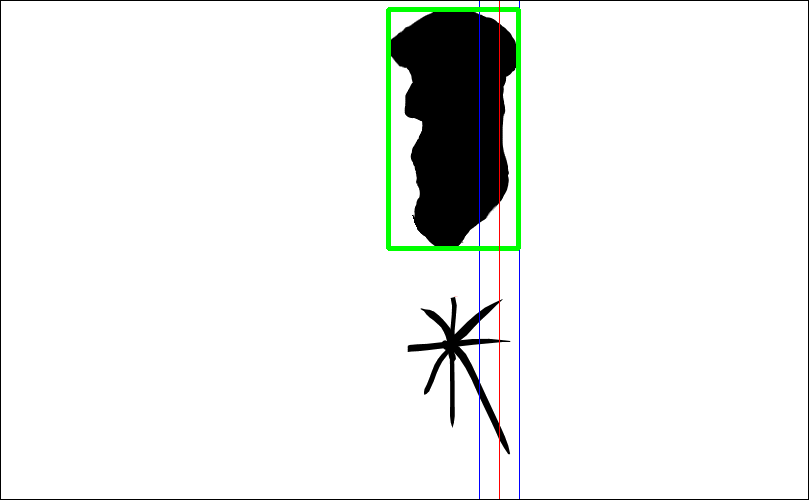
\includegraphics[angle=0,width=0.55\textwidth]{afsnit/afprovning/billeder/naive_losning/naiv_mass.png}
	       	\label{naiv_masse}}\hspace{1em}
	    \subfloat[Original]{
	        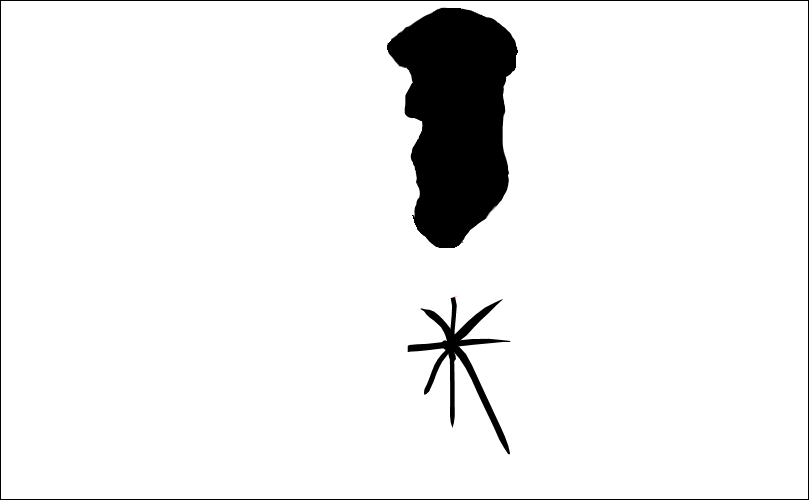
\includegraphics[angle=0,width=0.55\textwidth]{afsnit/afprovning/billeder/naive_losning/mass.png}
	       	\label{naiv_masse_original}}\hspace{1em}
		\label{masse}
\end{figure}
